\chapter{Data and Methodology}
\label{chap:data_methodology}

This section details the data sources and methodological approaches employed in this thesis. It begins by describing the primary data source, the ICIJ Offshore Leaks Database, outlining its structure, content, strengths, and limitations. Subsequently, it discusses the external datasets used to provide contextual information. Finally, it introduces a novel methodology utilizing agentic AI to enrich the classification of intermediaries within the icij dataset.

\section{The ICIJ Offshore Leaks Database}
\label{sec:3_1}

The empirical core of this thesis rests upon the International Consortium of Investigative Journalists (ICIJ) Offshore Leaks Database. This resource serves as the primary data source, acting as a valuable, albeit imperfect, "proxy" for the opaque universe of offshore finance (cf. EU, 2017). The general idea underpinning its use here is that while any direct numerical estimates derived solely from the leaks (e.g., total wealth hidden) will surely be biased due to the data's inherent incompleteness, the qualitative nature of the interactions captured within the data – the patterns of relationships between clients, intermediaries, and jurisdictions – appears more reliable for understanding the structure and dynamics of the offshore system.

The use of the ICIJ Offshore Leaks Database for this type of research is increasingly established. For example, Alstadsæter et al. (2019), Londoño-Vélez \& Ávila-Mahecha (2021), and Chang et al. (2023a; 2023b). 

Some direct network analysis, but not much. Most relevant for our purposes is the work of Chang et al. (2023a; 2023b), as well as a more direct network study (Kejriwal \& Dang, 2020) looking at the usual properties networks exhibit. They note:

"It was really unusual. The degree of fragmentation is something I have never seen before," said Kejriwal. "I'm not aware of any other network that has this kind of fragmentation."

The core datasets loaded for this analysis include:
\begin{itemize}
    \item \texttt{nodes-entities.csv}: Information on offshore companies, trusts, foundations.
    \item \texttt{nodes-officers.csv}: Details on individuals or companies acting in official capacities (directors, shareholders, beneficiaries).
    \item \texttt{nodes-intermediaries.csv}: Data on firms or individuals facilitating the creation and management of offshore structures.
    \item \texttt{nodes-addresses.csv}: Physical address information linked to other nodes.
    \item \texttt{nodes-others.csv}: Nodes not fitting the primary categories.
    \item \texttt{relationships.csv}: The edge list defining connections between nodes, including the type of relationship.
\end{itemize}
A multi-modal and multi-relational graph, that often involved dealing with it at various level of abstractions, and breaking the dimensionality of it. For example, most network algorithms cannot deal with multi-relational graphs (in fact, a tetrapartite graph composed of addresses, entities, officers and intermediaries!), built and formulated as traditional adjacency matrices operations, so often switching between different representations of the data, ranging from granular edge lists with the full ontology of the data model, to those squashed down into a format that can be represented as a single adjacency matrix (i.e. an edge list with only a single type of source- and end node).

Usual trick for dealing with bipartite graphs is projecting it down by connecting two nodes if they share a common node type, that one wants to eliminate. For example, for getting rid of address node type, relations like the following would be transformed as such:

Intermediary1 -- Address -- Intermediary2
-> Intermediary1 -- Intermediary2

This process can be done iteratively on all node types that one wants to eliminate:
Intermediary1 -- Entity -- Address -- Officer -- Intermediary2
-> Intermediary1 -- Intermediary2

And from here, traditional network algorithms calculating the likes of eigenvector centrality etc. can be applied.

Whenever moving between the different representations of the graph, will be made clear in the empirical section.


Note: ICIJ data is in principle directed, but in practice this is not especially important. Here, treated solely as an undirected graph.

\section{External Data Sources}

\label{sec:3_2}

To contextualize the patterns observed within the ICIJ data, several external data sources are employed.

A key resource is the Historical Tax Havens Database (HTHD) developed by Laffitte (2024). This dataset documents the historical evolution of "offshore legal architecture," tracking the adoption of specific legal technologies (e.g., banking secrecy, IBCs) across tax havens over time. This dataset will be utilized to explore whether specific patterns observed in the ICIJ data – such as the prevalence of certain offshore instruments or shifts in intermediary activity – align temporally with the historical innovations documented in the HTHD.

The World Justice Project (WJP) Rule of Law Index provides comprehensive country-level metrics on governance. Its specific use is to investigate potential correlations between the home country's rule of law environment and the patterns of specialization or network positioning observed among the intermediaries serving clients from that country.

VDEM (Varieties of Democracy) Regime Type Data will be used exactly analogously.

Data from the World Inequality Database (WID), specifically metrics on wealth inequality at the country level, will also be incorporated.  This serves primarily to see if we can confirm some of the comparative statics Alstadsæter and Zucman derive, trying to verify whether there's anything to their supply-side model.

\section{Using Agentic AI to Scrape Data on Intermediaries.}
\label{sec:3_3}

A significant challenge in utilizing the ICIJ data for the purposes of this thesis is that intermediaries are often classified generically within the database. To analyze the specific roles and potential influence of different types of intermediaries, as outlined in the typology adapted from the EU (2017) paper (see Section 2.1.4), a more granular classification is required. To achieve this classification at scale, an approach employing agentic AI is utilized.

The core idea is to use an AI agent loop to automate the process of gathering information about and classifying the intermediaries listed in the ICIJ data. The basic workflow is illustrated in Figure \ref{fig:agent_loop_placeholder}.

\begin{figure}[htbp]
    \centering
    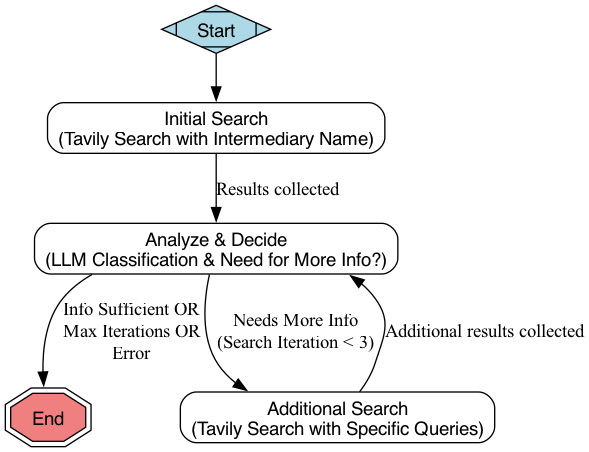
\includegraphics[width=0.8\textwidth]{agent_graph.png} % Assuming you have agent_graph.png
    \caption{Agent Setup for Intermediary Classification}
    \label{fig:agent_loop_placeholder}
\end{figure}

In brief, the process involves an AI agent orchestrating online searches for each intermediary identified in the ICIJ data. It begins with generic searches, reads and interprets the initial results, and then formulates more specific search queries based on the information discovered or identified as lacking. This iterative process involves up to three search queries per intermediary, scouring the top 15 most relevant web results identified through query-result embedding similarity using the Tavily Search API (though the tool is relatively generic and its specific choice is not critical to the methodology). This effectively replaces the time-consuming need for manual searching of the intermediaries.

Based on the information gathered, the AI agent then classifies the intermediary according to the EU (2017) typology (Tax Expert, Legal Expert, Administrator, Investment Advisor), adding a few additional relevant fields (e.g., specific job title). Crucially, the agent also provides a confidence score for its classification judgment, allowing for filtering or weighting in subsequent analyses.

There are a few obvious limitations associated with this approach that warrant discussion:

Temporal Misalignment: A primary concern is that all online searches are conducted based on information available today, whereas the ICIJ data pertains to activities that may have occurred years or even decades prior. This introduces two potential issues:
    \begin{enumerate}
        \item The process might be biased towards identifying intermediaries who are still active or have a significant online presence currently.
        \item It implicitly assumes that the role an intermediary plays today (as reflected online) is equivalent to the role they played at the time relevant to the ICIJ data.
    \end{enumerate}

Addressing the Limitations: While these issues are real, they are not prohibitive for their use in this thesis.
\begin{enumerate}
    \item Regarding the first point (bias towards current intermediaries), this primarily impacts the coverage or statistical power of the classification – we may only be able to confidently classify a subset (e.g., 50\%) of all intermediaries. This is acceptable, provided the unclassifiable intermediaries are not systematically different in ways that correlate with the research questions. The issue becomes problematic only if there is a systematic bias in identifiability across types (e.g., if it is inherently much harder to find information online about legal experts compared to tax experts due to differing needs for discretion or public visibility). The significant threat here is the bias in who provides public information - it will only be the intermediaries whose activities are not inherently illegal. A bias towards, in a sense, the least dangerous intermediaries as those being revealed.
    \item Regarding the second point (role stability), the assumption that roles remain consistent is arguably less problematic. Given the highly specialized nature of functions like tax advisory, legal structuring, administration, and investment management within the offshore context, and the considerable barriers to entry (qualifications, reputation, networks) for each, frequent switching between these core roles by individuals or firms seems relatively unlikely.
\end{enumerate}
In my view, it is the only pragmatically feasible method to do this given the constraints of this thesis.

To instruct the AI agent on how to perform the classification and the specific structure of the information to return, the following prompt template is utilized. This prompt defines the categories, provides keywords for guidance, and specifies the desired output fields. The agent's output for each intermediary is a structured data record, typically resembling a JSON object or a Python dictionary, which includes the fields detailed in the prompt.

\subsection*{Classification Prompt}
The core prompt provided to the AI agent for classification is as follows (where \texttt{\{intermediary\_name\}} and \texttt{\{log\_summary\_for\_classification\}} are dynamically inserted):
\begin{verbatim}
Classify the intermediary: {intermediary_name}

Based *only* on the information gathered in the following search log.
{log_summary_for_classification}

Classify this intermediary into ONE of these categories based on their
likely primary role in offshore activities:
- Tax Expert: Focuses on tax planning, compliance, advisory. Keywords:
  tax advisory, international tax, tax compliance, tax returns,
  transfer pricing, VAT, tax structuring.
- Legal Expert: Focuses on legal structuring, compliance, incorporation,
  representation. Keywords: legal services, corporate law, entity formation,
  incorporation, contracts, litigation, legal opinions, regulatory
  compliance, M&A legal, lawyer, attorney, solicitor.
- Administrator: Focuses on accounting, auditing, financial reporting,
  company administration. Keywords: accounting, bookkeeping, audit,
  financial statements, reporting, company secretarial, payroll,
  administration services, domiciliation, accountant, auditor.
- Investment Advisor: Focuses on managing financial assets and investments.
  Keywords: investment management, wealth management, asset management,
  portfolio management, financial planning, investment strategy,
  securities, funds, financial advisor.

Provide a structured classification including:
- classification (Enum: Tax Expert, Legal Expert, Administrator, Investment Advisor)
- role_muddled (bool: true if the role seems mixed or unclear)
- role_muddled_reasoning (str: explanation if role_muddled is true)
- is_individual (bool: based on the name and findings, is this likely a person?)
- job_title (str: inferred job title if possible, e.g., "Lawyer", "Accountant",
  "Director", or "Unknown")
- confidence (Enum: Low, High - Use Low if evidence is sparse, contradictory,
  or confidence in the source/relevance is low)
- justification (str: detailed reasoning for the classification, referencing the
  search log)
- key_evidence (list[str]: specific snippets or findings from the search
  results supporting the classification)

Analyze the content of the search results carefully. Prioritize information
directly describing the intermediary's services or professional role.
\end{verbatim}

\subsection*{Examples of Dynamic Search and Structured Output}

The agent's search process is dynamic. It begins with a general query (the intermediary's name) and, based on the retrieved information's relevance and completeness, may formulate up to two additional, more specific queries. For instance, if initial results for a company are vague, subsequent queries might include terms like "services offered" or "business activity." The classification is then made based on the entirety of the gathered search logs.

Sometimes it's just not possible to find anything useful, hence the confidence section. Any cases where `confidence` is low, they are excluded from the analysis sections.

The output for each intermediary is a structured record. While the `key\_evidence` field in the prompt requests specific snippets, for comprehensiveness in these examples, it contains the full, somewhat verbose, search log detailing each iteration of the dynamic search process.

The following examples illustrate this process and the resulting structured output, taken directly from the enrichment process. The first provides an example of where it's impossible to find clear information linked to the interemediary resulting in low confidence, while the second is a clear case of a legal expert.

\subsubsection*{Example 1: OPULENT OPAL HOLDINGS LIMITED}
\textbf{Dynamic Search Summary:}
\begin{itemize}
    \item \textbf{Iteration 0 Query:} `OPULENT OPAL HOLDINGS LIMITED`
    \item \textbf{Findings:} Results were ambiguous, pointing to "OPULENT OPAL CONSTRUCTION LIMITED," a subsidiary link to "Opal Holdings Pte Ltd" (itself a subsidiary of CapitaLand, suggesting a holding structure), and unrelated products (paint, home decor).
    \item \textbf{Iteration 1 Query:} `OPULENT OPAL HOLDINGS LIMITED primary business activities`
    \item \textbf{Findings:} Retrieved general information on Bank Secrecy Act compliance for businesses, potentially triggered by "holdings," and another mention of the CapitaLand subsidiary link.
    \item \textbf{Iteration 2 Query:} `OPULENT OPAL HOLDINGS LIMITED services offered`
    \item \textbf{Findings:} Largely irrelevant results (gemstones, furniture), again highlighting the difficulty in pinpointing specific services for this entity.
\end{itemize}

\textbf{Structured Output (Simplified Representation):}
\begin{itemize}
    \item \textbf{intermediary\_name:} OPULENT OPAL HOLDINGS LIMITED
    \item \textbf{classification:} Administrator
    \item \textbf{confidence:} Low
    \item \textbf{role\_muddled:} True
    \item \textbf{role\_muddled\_reasoning:} "The role is muddled as the search results are ambiguous and could indicate construction, holding company activities, or other possibilities. There is no clear indication of their primary business activities."
    \item \textbf{is\_individual:} False
    \item \textbf{job\_title:} Unknown
    \item \textbf{justification:} "The search results provide limited information about OPULENT OPAL HOLDINGS LIMITED. One result mentions 'OPULENT OPAL CONSTRUCTION LIMITED' which suggests involvement in construction, potentially as a specialty trade contractor. Another result indicates that 'Opal Holdings Pte Ltd' is a subsidiary of CapitaLand, implying a holding company structure. The lack of direct evidence about their services or role leads to a low confidence classification as an administrator, potentially involved in company administration or holding activities."
    \item \textbf{key\_evidence (Full Search Log):} (Content of the JSON-like string representing the three search iterations and their results, as provided in the original example, would be detailed here. For brevity, it is summarized above and omitted in this representation.)
\end{itemize}

\subsubsection*{Example 2: Cheo Yeoh \& Associates}
\textbf{Dynamic Search Summary:}
\begin{itemize}
    \item \textbf{Iteration 0 Query:} `Cheo Yeoh \& Associates`
    \item \textbf{Findings:} Immediately yielded relevant results identifying the entity as "CHEO YEOH \& ASSOCIATES LLC," a Singapore-based company providing legal services, with details on its registration and directors.
    \item \textbf{Iteration 1 Query:} `Cheo Yeoh \& Associates services`
    \item \textbf{Findings:} Reinforced the legal nature, with results like "Cheo Yeoh \& Associates provides legal services" and official listings specifying "LEGAL ACTIVITIES."
    \item \textbf{Iteration 2 Query:} `Cheo Yeoh \& Associates client testimonials` (or similar refinement if needed)
    \item \textbf{Findings:} Could uncover legal case mentions, lawyer profiles, or further business directory listings, solidifying its role. (The provided log indicates successful identification primarily from the first two iterations).
\end{itemize}

\textbf{Structured Output (Simplified Representation):}
\begin{itemize}
    \item \textbf{intermediary\_name:} Cheo Yeoh \& Associates
    \item \textbf{classification:} Legal Expert
    \item \textbf{confidence:} High
    \item \textbf{role\_muddled:} False
    \item \textbf{role\_muddled\_reasoning:} (Empty or N/A)
    \item \textbf{is\_individual:} False
    \item \textbf{job\_title:} Lawyer (Implicitly, as a law firm)
    \item \textbf{justification:} "Cheo Yeoh \& Associates LLC provides legal services in Singapore. The company's principal activity is LEGAL ACTIVITIES (EXCLUDING ONLINE MARKETPLACES). Johnny Cheo is a Director at the firm. The firm has been operating for 23 years. The search results consistently point to legal services."
    \item \textbf{key\_evidence (Full Search Log):} (Content of the JSON-like string representing the search iterations and their results, as provided in the original example, would be detailed here. For brevity, it is summarized above and omitted in this representation.)
\end{itemize}\section{Use of LLMs}

\section{Use of LLMs in the Broader Paper}
\label{sec:3_4}

LLMs have also been used to polish the text of this thesis and used for idea generation.

Used Google Gemini models mainly, with the seed configured to 42:
\begin{itemize}
    \item gemini-2.5-pro-preview-05-06
    \item gemini-2.5-pro-experimental-03-25
\end{itemize}

